\documentclass[12pt, a4paper, oneside]{article}\usepackage[]{graphicx}\usepackage[]{color}
%% maxwidth is the original width if it is less than linewidth
%% otherwise use linewidth (to make sure the graphics do not exceed the margin)
\makeatletter
\def\maxwidth{ %
  \ifdim\Gin@nat@width>\linewidth
    \linewidth
  \else
    \Gin@nat@width
  \fi
}
\makeatother

\definecolor{fgcolor}{rgb}{0.345, 0.345, 0.345}
\newcommand{\hlnum}[1]{\textcolor[rgb]{0.686,0.059,0.569}{#1}}%
\newcommand{\hlstr}[1]{\textcolor[rgb]{0.192,0.494,0.8}{#1}}%
\newcommand{\hlcom}[1]{\textcolor[rgb]{0.678,0.584,0.686}{\textit{#1}}}%
\newcommand{\hlopt}[1]{\textcolor[rgb]{0,0,0}{#1}}%
\newcommand{\hlstd}[1]{\textcolor[rgb]{0.345,0.345,0.345}{#1}}%
\newcommand{\hlkwa}[1]{\textcolor[rgb]{0.161,0.373,0.58}{\textbf{#1}}}%
\newcommand{\hlkwb}[1]{\textcolor[rgb]{0.69,0.353,0.396}{#1}}%
\newcommand{\hlkwc}[1]{\textcolor[rgb]{0.333,0.667,0.333}{#1}}%
\newcommand{\hlkwd}[1]{\textcolor[rgb]{0.737,0.353,0.396}{\textbf{#1}}}%

\usepackage{framed}
\makeatletter
\newenvironment{kframe}{%
 \def\at@end@of@kframe{}%
 \ifinner\ifhmode%
  \def\at@end@of@kframe{\end{minipage}}%
  \begin{minipage}{\columnwidth}%
 \fi\fi%
 \def\FrameCommand##1{\hskip\@totalleftmargin \hskip-\fboxsep
 \colorbox{shadecolor}{##1}\hskip-\fboxsep
     % There is no \\@totalrightmargin, so:
     \hskip-\linewidth \hskip-\@totalleftmargin \hskip\columnwidth}%
 \MakeFramed {\advance\hsize-\width
   \@totalleftmargin\z@ \linewidth\hsize
   \@setminipage}}%
 {\par\unskip\endMakeFramed%
 \at@end@of@kframe}
\makeatother

\definecolor{shadecolor}{rgb}{.97, .97, .97}
\definecolor{messagecolor}{rgb}{0, 0, 0}
\definecolor{warningcolor}{rgb}{1, 0, 1}
\definecolor{errorcolor}{rgb}{1, 0, 0}
\newenvironment{knitrout}{}{} % an empty environment to be redefined in TeX

\usepackage{alltt} % Paper size, default font size and one-sided paper
%\graphicspath{{./Figures/}} % Specifies the directory where pictures are stored
%\usepackage[dcucite]{harvard}
\usepackage{rotating}
\usepackage{amsmath}
\usepackage{setspace}
\usepackage{pdflscape}
\usepackage[flushleft]{threeparttable}
\usepackage{multirow}
\usepackage[comma, sort&compress]{natbib}% Use the natbib reference package - read up on this to edit the reference style; if you want text (e.g. Smith et al., 2012) for the in-text references (instead of numbers), remove 'numbers' 
\usepackage{graphicx}
%\bibliographystyle{plainnat}
\bibliographystyle{agsm}
\usepackage[colorlinks = true, citecolor = blue, linkcolor = blue]{hyperref}
%\hypersetup{urlcolor=blue, colorlinks=true} % Colors hyperlinks in blue - change to black if annoying
%\renewcommand[\harvardurl]{URL: \url}
\IfFileExists{upquote.sty}{\usepackage{upquote}}{}
\begin{document}
\title{Textbook Examples}
\author{Rob Hayward} 
\date{\today}
\maketitle
\section{Box 3.3, p. 66}

The following equation for a demand curve

$$Q = 60 - 15P + P^2$$

\begin{knitrout}
\definecolor{shadecolor}{rgb}{0.969, 0.969, 0.969}\color{fgcolor}
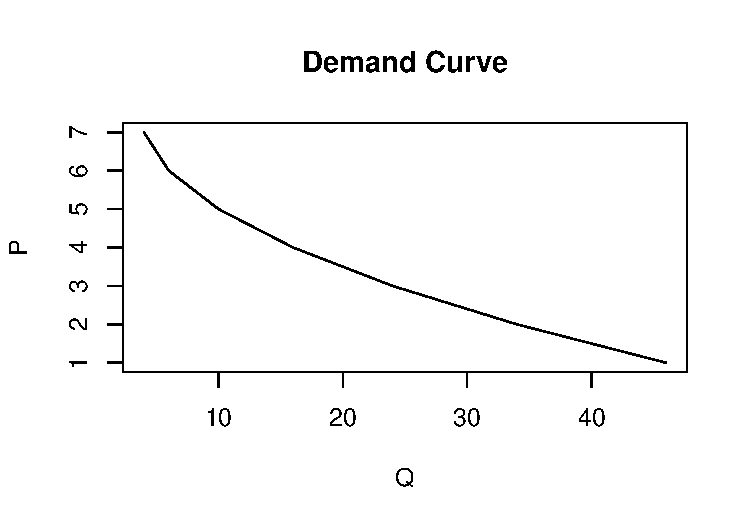
\includegraphics[width=\maxwidth]{figure/table} 

\end{knitrout}

$$p_{ed} = \frac{\text{proportionate change in } Q}{\text{proportionate change in } P}$$
Remember 
$$\text{proportionate change } x = \frac{\Delta x}{x} \times 100$$

so, for a very small change in price 

$$p_{ed} = \frac{dQ}{dP} \times \frac{P}{Q}$$

$$\frac{dQ}{dP} = -15 + 2P$$

Therefore, what is the elasticity at the price of 3? 

$$P_{ed} = \frac{dQ}{dP} \times \frac{P}{Q}$$

$$-15 + 2P \times \frac{3}{24}$$

$$ -15 + 6 = -9$$

$$ -9 \times \frac{3}{4} = -\frac{9}{8}$$

This is elastic.

\section{Box 4.1 p. 102}
Consumer Utility is 

$$TU = 60Q - 4Q^2$$

$$MU = \frac{dTU}{dQ} = 60 - 8Q$$

\begin{knitrout}
\definecolor{shadecolor}{rgb}{0.969, 0.969, 0.969}\color{fgcolor}
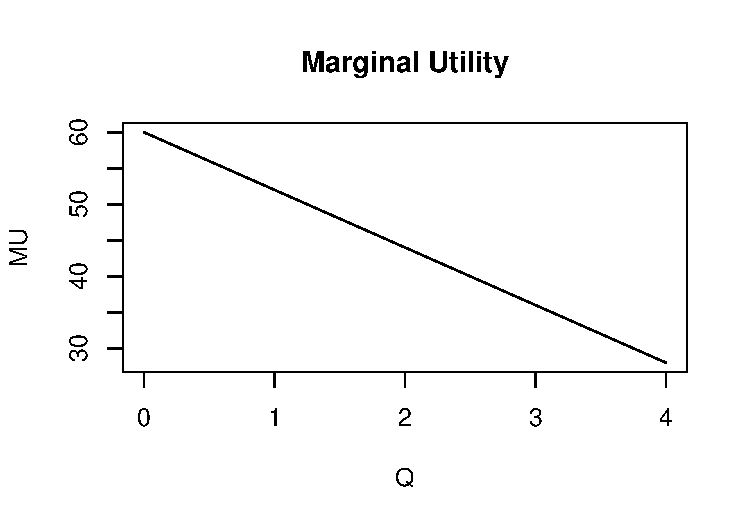
\includegraphics[width=\maxwidth]{figure/MU} 

\end{knitrout}


\section{Box 5.4, P. 138}
This is discussed in the lecture on calculus and is in the lecture slides.

\section{Box 5.9 p. 166}
Total Revenue
$$TR = 48Q - Q^2$$
Total Cost 
$$TC = 12 + 16Q +3Q^2$$
There is a table in the textbook that will calculate the costs and revenues for each of the quantities.  As Profit is the difference between total cost and total revenue, finding the maximum profit that way is relatively easy. 

However, it is also possible to use the fact that profits will be maximised at the point where marginal revenue equal marginal cost. Remember that marginal revenue is the derivative of total revenue and marginal cost is the derivative of total cost. 
Marginal Revenue
$$ MR = \frac{d(TR)}{d(Q)} = 48 - 2Q$$
Marginal Cost
$$MC = \frac{d(TC)}{d(Q)} = 16 +6Q$$

Set $MR = MC$

$$48 - 2Q = 16 + 6Q$$

Solving for Q
$$32 = 4Q$$

or
$$Q = 4$$

Now substitute 4Q into the equation for Total Profit

$$TP = TR - TC$$

or 

$$TP = 48Q - Q^2 - (12 + 16Q +3Q^2)$$
$$TP = -12 + 32Q - 4Q^2$$
 substitute $Q = 4$
 
$$TP = -12 +(32 \times 4) - 4(4^2)$$
$$TP = 52$$


\end{document}
